\renewcommand*{\mypath}{superapp}%
\graphicspath{ {\mypath/images/} }

\doctitle{Lorenzo Affetti}{lorenzo.affetti@polimi.it}

\section{Introduzione}
Lo scopo dell'applicazione SuperApp è quello di mettere in atto una collaborazione tra quattro giocatori attraverso diverse modalità di gioco.
Ogni giocatore della squadra gioca su un tablet diverso, uno \textit{slave}. Il gioco necessita di un ulteriore tablet, il \textit{master}, che non verrà utilizzato da nessun giocatore, ma che fornirà informazioni di massima sulla partita in corso e scandirà le partite e le manche di gioco.

I dispositivi comunicano per mezzo di una connessione \textit{Bluetooth}. Un disegno di massima delle posizioni dei tablet è fornito in figura \ref{fig:tablet5}.

\begin{figure}[h!]
\centering{
\includegraphics[width=\textwidth]{tablets.png}}
\caption{I cinque tablet}
\label{fig:tablet5}
\end{figure}

L'applicazione comprende tre diversi giochi:

\begin{itemize}
\item \textit{Trova l'Intruso}: I giocatori devono, appunto, trovare l'intruso. Ad un certo numero di risposte esatte consecutive (configurabile) la logica di gioco si inverte (vengono dati feedback sonori e visivi) e il gioco diventa, quindi, trova il \textit{non} intruso. Questo gioco può essere lanciato in quattro diverse modalità: trova l'intruso per colore, \textit{ancora-colore} (come la modalità per colore, con la differenza che le immagini vengono mostrate in bianco e nero all'inversione di gioco), direzione e forma. 
\item \textit{Ordina dal Più Piccolo al Più Grande}: I giocatori devono ordinare quattro oggetti dal più piccolo al più grande o viceversa.
\item \textit{Costruisci la Torre}: I giocatori devono completare una torre composta da quattro oggetti giocando a turno.
\end{itemize}

In ognuno dei tre giochi l'applicazione sottopone agli utenti delle immagini che si muovono con velocità variabile su dei nastri trasportatori.

Ogni \textit{partita} è composta da un numero di \textit{manche} (o anche \textit{stage}) configurabile. Il completamento di tutte le manche porta alla vittoria del gruppo. I punteggi sono sempre cumulativi dell'intera squadra.

\section{Struttura Generale}
% - i vari pattern di comunicazione
% TODO diagramma di interazione back <-> front (con tanto di eventi)

\begin{figure}[h!]
\centering{
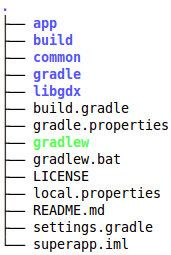
\includegraphics{tree_root.png}}
\caption{La struttura del progetto (profondità 1)}
\label{fig:tree_root}
\end{figure}

Il codice sorgente dell'applicazione è suddiviso in tre moduli (figura \ref{fig:tree_root}). Il modulo \code{app} contiene il backend, comprensivo di logica di gioco e di comunicazione, e il frontend dell'applicazione. Il modulo \code{libgdx} contiene le parti più interattive dell'applicazione e cioè quelle dei nastri trasportatori. Infine, il modulo \code{common} contiene moduli privi di dipendenze dal framework di Android e usati in ambedue i precedenti moduli.

Come già accennato, SuperApp è divisa in tre diversi giochi di cui il primo è disponibile in quattro modalità diverse (in realtà, anche il secondo, tuttavia la logica di gioco rimane invariata tra di esse, ciò che varia è solo l'ordinamento delle quattro immagini iniziali). Per questo motivo, quasi ogni classe costituente il nucleo della logica di gioco (si veda \ref{subsec:logic}) e diversi \textit{fragment} (si veda \ref{subsec:activities}) segue il particolare schema di ereditarietà illustrato in figura \ref{fig:hierarchy}, a parte sporadiche eccezioni che, però, sono facilmente comprensibili a una prima lettura del codice (per esempio, abbiamo \code{Slave1Color} e \code{Slave1ColorAgain}, ma solo un \code{MasterColor} poiché il ruolo del \textit{master} nelle due modalità non cambia).

\begin{figure}[h!]
\centering{
\includegraphics[width=\textwidth]{hierarchy.png}}
\caption{Lo schema di ereditarietà generale}
\label{fig:hierarchy}
\end{figure}

Gli elementi costitutivi dell'intera applicazione sono:

\begin{description}
\item[i \textit{Controller}] rappresentano la logica di gioco e mantengono lo stato del gioco;
\item[i \textit{Tile}] o tesserini, costituiscono il modello dell'applicazione (si veda la classe \code{it.playfellas.superapp.tiles.Tile} nel modulo \code{common}). Sono le immagini che l'utente toccherà per dare delle risposte;
\item[la \textit{UI}] mostra il gioco all'utente e raccoglie le sue azioni;
\item[i \textit{Presenter}] interpretano le azioni dell'utente fornite dalla \textit{UI} fornendole ai \textit{Controller}. In base al responso ottenuto, vanno a informare la \textit{UI} dei cambiamenti da apportare.
\item[il \textit{Bus}] permette la comunicazione per mezzo di \textit{eventi} tra gli elementi costitutivi dell'applicazione (in locale) e tra i dispositivi coinvolti (in remoto, tramite \textit{Bluetooth}). Per maggiori informazioni riguardo alla comunicazione, si veda la sezione \ref{subsec:tenbus}.
\end{description}

Il diagramma in figura \ref{fig:components} mostra i vari componenti di SuperApp e la loro interazione ad alto livello su un dispositivo \textit{slave}, quello che mostra il maggior numero di interazioni con l'utente. Il diagramma fornito non vuole essere esaustivo di tutti i possibili messaggi scambiati tra i moduli, bensì vuole chiarire li idee al lettore e fornire un'idea di massima delle interazioni tra le classi.

\begin{figure}[h!]
\centering{
\includegraphics[width=\textwidth]{components.png}}
\caption{Le componenti di SuperApp su uno \textit{slave}}
\label{fig:components}
\end{figure}


\section{Backend}

\subsection{Il TenBus}
\label{subsec:tenbus}
Prima di spiegare il funzionamento di qualsiasi altro componente di SuperApp è necessario introdurre il \code{TenBus}, parte del package \code{it.playfellas.superapp.network}. Questa classe è quella che permette a tutte le componenti del sistema di comunicare tra di loro -- sia in remoto che in locale -- per mezzo della trasmissione di \textit{eventi}. Il \code{TenBus} è un \textit{wrapper} attorno al famoso \textit{bus} ad eventi \textbf{Otto} (\url{http://square.github.io/otto/}).

Dopo aver ottenuto un'istanza del \code{TenBus} tramite il metodo statico \code{get}, un oggetto può \code{post}are \code{NetEvent} oppure \code{InternalEvent}. I primi verranno inviati in remoto sul canale \textit{Bluetooth}, i secondi verranno propagati in locale usando l'originale Otto. Gli eventi sono di molteplici tipi e le loro classi sono contenute nel package \code{it.playfellas.superapp.events}. La generazione di questi ultimi è accentrata nella \code{EventFactory}.

Se un oggetto volesse ricevere degli eventi, dovrà semplicemente invocare il metodo \code{register} passando un qualsiasi oggetto (anche \code{this}) che abbia registrato dei metodi tramite l'annotazione \code{@Subscribe}. I methodi annotati devono accettare in ingresso un oggetto di tipo uguale all'evento interessato e ritornare un valore \code{void}.

Il \code{TenBus} offre anche i metodi \code{attach} e \code{detach} per permettere lo scambio di eventi in remoto. Per il funzionamento dettagliato della connessione \textit{Bluetooth} (inizializzazione, chiusura) si veda il codice.

Le classi \code{BTThread} e \code{Peer} (e quelle che le estendono) sono volutamente invisibili all'esterno del package \code{network}, l'unico punto d'accesso alla rete per un oggetto esterno è il \code{TenBus}.

\subsection{La Logica di Gioco}
\label{subsec:logic}
% la GameHistory?

\begin{figure}[h!]
\centering{
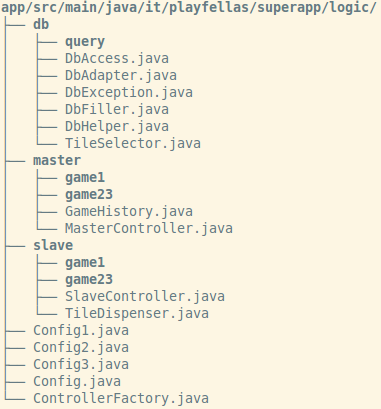
\includegraphics{tree_logic.png}}
\caption{La struttura del package \texttt{it.playfellas.superapp.logic}}
\label{fig:tree_logic}
\end{figure}

Gli elementi fondamentali della logica di gioco sono contenuti nel package \code{it.playfellas.superapp.logic} (per una struttura del package si veda figura \ref{fig:tree_logic}):

\begin{description}
\item[\textbf{I Dispenser}]\hfill\\
    Sostanzialmente sono, come chiarisce la \textit{signature} della classe \code{it.playfellas.superapp.logic.slave.TileDispenser}, degli \code{Iterator<Tile>}. Quello che un \textit{dispenser} fa, infatti, è fornire un nuovo \textit{tile} ad ogni invocazione del metodo \code{next}. Ogni modalità di gioco ha un suo particolare \textit{dispenser} (il gioco 1 ne ha, invece, due: uno normale e l'altro per l'inversione di gioco), il quale interroga il \textit{database} dell'applicazione (che contiene solo \textit{tile}) per ottenere un insieme di tesserini. Questi ultimi verranno forniti tramite il metodo \code{next} secondo logiche proprie del \textit{dispenser} stesso. Per indagare le logiche specifiche si veda il codice sorgente degli specifici \code{TileDispenser} contenuti nei package \code{it.playfella.superapp.logic.slave.game1} e \code{game23};
\item[\textbf{I Master Controller}]\hfill\\
    I \textit{controller} rappresentano la logica di logico. Ogni azione che l'utente compie per mezzo di un gesto sullo schermo del tablet viene interpretata dalla parte di \textit{UI} e viene passata ad un \textit{controller} che saprà interpretarla e fornire una risposta in base allo stato attuale della partita. I \textit{master}, nello specifico, sono quelli che mantengono lo stato globale della partita (per esempio: il punteggio, i giocatori, ecc.) e danno inizio alle partite sugli \textit{slave} (si veda il metodo \code{beginStage}) fornendo, a volte, informazioni condivise (per esempio, nel gioco 1, il colore/forma/direzione base; nei giochi 2 e 3, le quattro \textit{tile} di base)). Oltre a dare inizio alle partite, ne scandiscono ogni fase, come l'inizio e la fine della partita stessa e l'inizio e la fine delle manche che la compongono.
\item[\textbf{Gli Slave Controller}]\hfill\\
    Gli \textit{slave} attendono che i \textit{master} trasmettano gli eventi di inizio/fine partita e inizio/fine manche per poter dare inizio al gioco vero e proprio. Essi istanziano i \textit{dispenser} per ottenere i prossimi \textit{tile} da fornire agli utenti. Essi contengono anche la parte di logica di gioco riguardante l'esattezza o meno di un \textit{tile} date le sue caratteristiche (vedi metodo \code{isTileRight}). Quest'ultima informazione è quella che verrà trasmessa tramite eventi al \textit{master} che deciderà, di conseguenza, se incrementare, azzerare o altro il punteggio complessivo. Ogni \code{SlaveController} fornisce anche un metodo \code{nextTile} che viene usato dalla \textit{UI} per ottenere il prossimo \textit{tile} e mostrarlo all'utente, posizionandolo nel momento giusto sul nastro trasportatore (si veda \code{it.playfellas.superapp.ui.slave.DisposingService}).
\end{description}

\subsubsection{La Partita}
Come precedentemente detto, la partita è articolata in un numero configurable di stage. Ognuno di essi prevede un punteggio massimo configurabile. Al raggiungimento di tale punteggio, lo stage termina e si dà inizio allo stage successivo. Quando tutti gli stage sono stati completati, la partita finisce.

La scansione della partita nelle suddette fasi è determinata dal \code{MasterController}. Esso invia, tramite il \code{TenBus}, un evento \code{StartGameEvent} (in realtà, viene inviato un evento che estende quella classe. Per esempio: \code{StartGame1Color}, oppure \code{StartGame2Event}, ecc.). Alla ricezione dell'evento, ogni \textit{slave} reagisce mostrando la schermata di gioco all'utente. A questo punto, il \textit{master} procede per stage fino al loro esaurimento.

Viene inviato un \code{BeginStageEvent} e lo stage ha inizio. Quando il punteggio massimo viene raggiunto, il \textit{master} invia un \code{EndStageEvent} seguito da un \code{BeginStageEvent} in caso vi sia un altro stage da giocare, altrimenti viene inviato un \code{EndGameEvent}.

In figura \ref{fig:game_flow}, viene rappresentata la successione di eventi che porta alla fine della partita.

\begin{figure}[h!]
\centering{
\includegraphics[width=\textwidth]{game_flow.png}}
\caption{La partita}
\label{fig:game_flow}

\end{figure}


\section{Frontend}

\subsection{Le Activity e i Fragment}
\label{subsec:activities}
In questa sezione riportiamo un elenco delle \textit{activity} e dei \textit{fragment} e le loro principali mansioni.
Per il codice sorgente si faccia riferimento al package \code{it.playfellas.superapp.ui}.

\begin{description}
\item[MainActivity] è il punto di accesso dell'applicazione, permette di scegliere tra \textit{master} e \textit{slave};
\item[master.MasterActivity] permette la scelta tra i diversi giochi (1, 2 e 3);
\item[master.GameActivity] è l'\textit{activity} in cui avviene la partita nel \textit{master}. Contiene i seguenti \textit{fragment}:
    \begin{description}
        \item[SettingsFragment] permette di configurare il gioco corrente;
        \item[GameFragment] mostra lo stato della partita (stage, punteggio, foto dei giocatori, ecc.). Istanzia il giusto (per la modalità di gioco corrente) \code{GamePresenter} che a sua volta istanzia il giusto \code{MasterController}.
    \end{description}
\item[master.bluetooth.BluetoothActivity] permette l'associazione dei dispositivi.
\item[master.bluetooth.FastStartActivity] permette l'avvio rapido del \textit{master} riassociando gli ultimi dispositivi connessi.
\item[slave.SlaveActivity] \textit{activity} in cui lo \textit{slave} aspetta di venir scelto dal \textit{master} come giocatore della partita tramite associazione \textit{Bluetooth};
\item[slave.GameActivity] è l'\textit{activity} in cui avviene la partita nello \textit{slave}. Tramite la ricezione degli eventi che estendono \code{StartGameEvent}, determina la modalità di gioco corrente e sceglie, di conseguenza, il giusto \textit{fragment} da mostrare. Contiene i seguenti \textit{fragment}:
    \begin{description}
        \item[PhotoFragment] l'utente può scattarsi una foto da utilizzare come \textit{avatar} durante la partita;
        \item[SlaveGameFragment] contiene i nastri trasportatori e i \textit{tiles} (vedi sezione \ref{subsec:libgdx}). Istanzia i nastri trasportatori e lo \code{SlavePresenter} (che, come sul \textit{master}, istanzia lo \code{SlaveController}) in base alla modalità di gioco corrente.
    \end{description}
\end{description}

Per l'istanziazione dei \textit{controller} si faccia riferimento a \code{it.playfellas.superapp.logic.ControllerFactory}.

\subsection{I Nastri}
\label{subsec:libgdx}
Il modulo del progetto che gestisce la visualizzazione e lo scorrimento dei nastri e la rappresentazione e animazione dei \textit{tile} è \code{libgdx}. \textbf{LibGDX} (\url{https://libgdx.badlogicgames.com/features.html}) è un framework Java che utilizza \textbf{OpenGL} (\url{https://www.opengl.org/}) per la renderizzazione video. Il risultato della scelta di questo framework è un miglioramento sia nella fluidità delle animazioni, che nell'occupazione della memoria del dispositivo da parte dell'applicazione rispetto all'utilizzo dell'\code{ObjectAnimator} standard di Android.

\textit{LibGDX} racchiude i concetti più comuni dei framework di renderizzazione grafica. Troviamo infatti la \textit{scena}, il "luogo" in cui avvengono le animazioni, e gli \textit{sprite}, immagini bidimensionali dotate di posizione, texture (la loro immagine), altezza e larghezza.

Gli elementi costitutivi del modulo \code{libgdx} sono:

\begin{description}
    \item[la Scene] la \textit{scena} del gioco;
    \item[i Conveyor] sono i nastri trasportatori, su cui vengono posati i \textit{tile}. Essi possono essere di diversi tipi. Troviamo infatti \code{MovingConveyor}, \code{SizeConveyor} e \code{TowerConveyor}.\\
        Bisogna notare che gli ultimi due non sono propriamente nastri trasportatori, in quanto sono statici e vengono utilizzati nei giochi 2 e 3 rispettivamente.
    \item[le TileRepr] sono dei \textit{wrapper} intorno ad un \code{Tile} e un \code{SimpleSprite}. Essi sono la rappresentazione concreta di un \textit{Tile} (quello del modello dell'applicazione). La corrispondenza \code{TileRepr} (rappresentazione), \code{Tile} (modello) è talmente stretta e semanticamente equivalente che, da ora in poi, utilizzeremo i due termini in modo intercambiabile.
\end{description}

Ciò che avviene ad ogni frame di visualizzazione è l'esecuzione del metodo \code{render} della \code{Scene}, il quale aggiunge ogni \textit{sprite} presente nella scena ad un \textit{batch} di renderizzazione, dopo averne aggiornato posizioni, texture e dimensioni. Il \textit{batch} così generato, contenente una matrice di pixel che rappresenta il "disegno" degli \textit{sprite} aggiunti, viene renderizzato tramite l'invocazione di \code{batch.end()}.

Per comprendere cosa si intende per "aggiornamento" di uno \textit{sprite}, si pensi alla sua posizione: per far muovere un nastro o un \textit{tile}, infatti, è necessario cambiare la sua posizione pixel per pixel ad ogni frame di rappresentazione (si vedano i metodi \code{update} nelle classi che estendono \code{Conveyor}).

